\documentclass{beamer}
\mode<presentation>
{
  \usetheme{default}      % or try Darmstadt, Madrid, Warsaw, ...
  \usecolortheme{default} % or try albatross, beaver, crane, ...
  \usefonttheme{default}  % or try serif, structurebold, ...
  \setbeamertemplate{navigation symbols}{}
  \setbeamertemplate{caption}[numbered]
} 

\usepackage[english]{babel}
\usepackage[utf8x]{inputenc}
\usepackage{scrextend}
\usepackage{graphicx}
\usepackage{booktabs}
\usepackage{adjustbox}
\usepackage{marvosym}
\usepackage{amsmath}
\usepackage{float}
\graphicspath{ {./images} }

\newcommand*{\Comb}[2]{{}^{#1}C_{#2}}%

\title[Pres]{Methods and Tools for the Analysis of Legacy Software
Systems\\
Report 1. Logical dependencies extraction - impact factors.
 }
\author{Stana Adelina Diana}
\institute{Computer Science and Engineering Department\\
"Politehnica" University of Timisoara}
\date{May, 2021}

\begin{document}

\begin{frame}
  \titlepage
\end{frame}

%%%%%%%%%%%%%%%%%%%%%%%%%%%%%%%%%%%%%%%%%%
\section{Presentation of the research topic}
 \begin{frame}
\frametitle{Presentation of the research topic}
The goal of the thesis is to develop methods for analyzing legacy software systems by using historical information extracted from the versioning systems.
We divided our work into two main parts

\begin{itemize}
\item \textbf{historical information collection and filtering}
\item usage of the collected information in order to analyze the software systems
\end{itemize}

\end{frame}

%%%%%%%%%%%%%%%%%%%%%%%%%%%%%%%%%%%%%%%%%%

 \begin{frame}
\frametitle{Structural dependencies}
\begin{block}{Definition}
Structural dependencies are the result of \textit{source code analysis} and can be extracted from: members, call parameters, local variables. 
\end{block}

\begin{center}
     \begin{figure}
	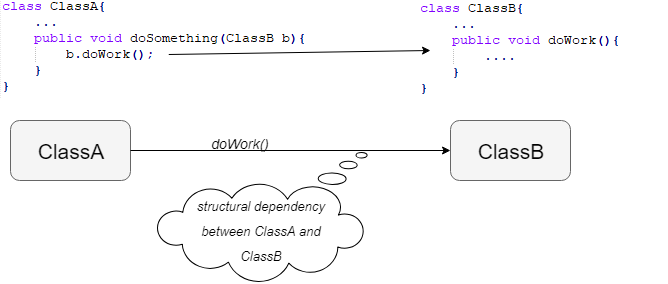
\includegraphics[width=\textwidth]{structural_dep.png}
	\caption{\label{fig:fig}Example of structural dependency between two classes}
     \end{figure}
\end{center}

\end{frame}

%%%%%%%%%%%%%%%%%%%%%%%%%%%%%%%%%%%%%%%%%%%

 \begin{frame}
\frametitle{Logical dependencies}
\begin{block}{Definition}
 Logical dependencies are the result of \textit{software history analysis} and can reveal relationships that are not present in the source code code (structural dependencies).
\end{block}

\begin{center}
     \begin{figure}
	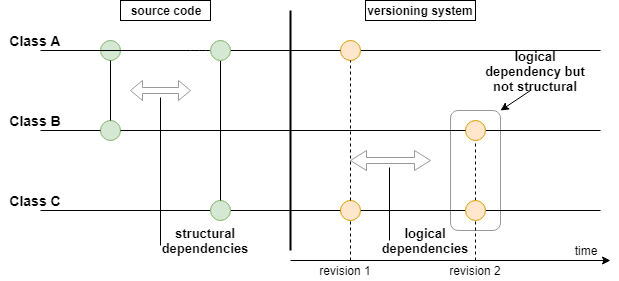
\includegraphics[width=\textwidth]{fig1.png}
	\caption{\label{fig:fig1}Example of logical and structural dependencies}
     \end{figure}
\end{center}

\end{frame}

%%%%%%%%%%%%%%%%%%%%%%%%%%%%%%%%%%%%%%%%%%%
 \begin{frame}
\frametitle{From co-changing pairs to logical dependencies}
The information extracted from the versioning system is under the form of pairs of classes that record co-changes (co-changing pairs). A co-changing pair that passes the filtering steps is considered a logical dependency.

\begin{center}
     \begin{figure}
	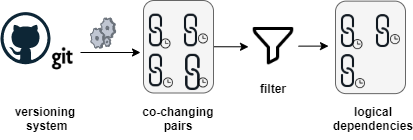
\includegraphics[width=\textwidth]{co-change_to_ld.png}
	\caption{\label{fig:fig1}Co-changing pairs extraction and filtering.}
     \end{figure}
\end{center}
\end{frame}


%%%%%%%%%%%%%%%%%%%%%%%%%%%%%%%%%%%%%%%%%%%
 \begin{frame}
\frametitle{Tool for measuring software dependencies}
We built a tool that identifies logical and structural dependencies from software systems.
\begin{center}
     \begin{figure}
	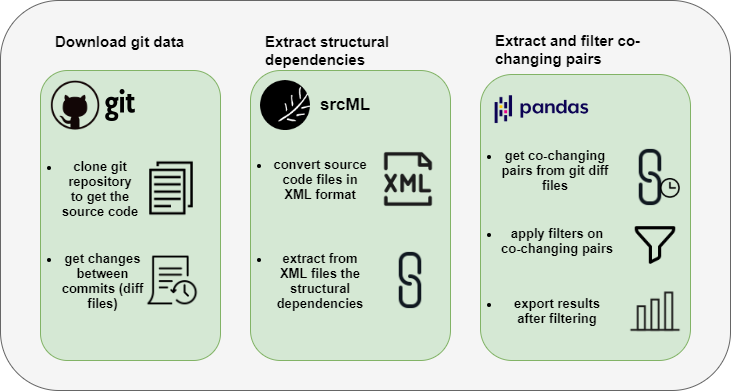
\includegraphics[width=\textwidth]{tool_workflow.png}
	\caption{\label{fig:fig1}Tool functionalities.}
     \end{figure}
\end{center}
\end{frame}


%%%%%%%%%%%%%%%%%%%%%%%%%%%%%%%%%%%%%%%%%%%
 \begin{frame}
\frametitle{Extracting co-changing pairs}
Git clone and diff commands were used to acquire the needed information for co-changing pairs extraction.
\begin{center}
     \begin{figure}
	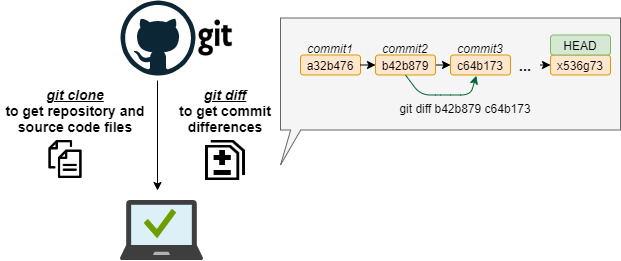
\includegraphics[width=\textwidth]{gitdata.png}
	\caption{\label{fig:fig1} Commands used to download the required data.}
     \end{figure}
\end{center}
\end{frame}

%%%%%%%%%%%%%%%%%%%%%%%%%%%%%%%%%%%%%%%%%%%
 \begin{frame}
\frametitle{Extracting co-changing pairs (cont.)}
The diff file contains all the changes between two commits.
\begin{center}
     \begin{figure}
	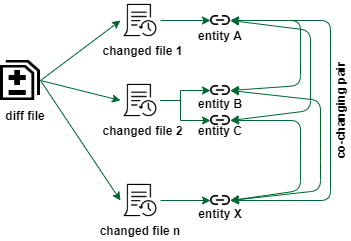
\includegraphics[scale=0.65]{cochange_extract.png}
	\caption{\label{fig:fig1}Co-changing pairs extraction from the versioning system.}
     \end{figure}
\end{center}
\end{frame}

%%%%%%%%%%%%%%%%%%%%%%%%%%%%%%%%%%%%%%%%%%%
 \begin{frame}
\frametitle{Co-changing pairs filtering}
The filters used are the commit size filter, occurrence filter, and connection strength filter. 
\begin{center}
     \begin{figure}
	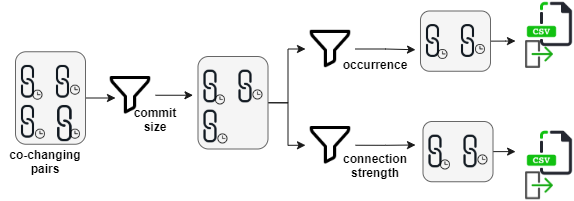
\includegraphics[width=\textwidth]{co-change_filtering.png}
	\caption{\label{fig:fig1}Co-changing pairs filtering.}
     \end{figure}
\end{center}
To see how the filters impact the results obtained, we studied 27 open-source projects and reported the results.
\end{frame}

%%%%%%%%%%%%%%%%%%%%%%%%%%%%%%%%%%%%%%%%%%%

\begin{frame}
\frametitle{Open source projects studied}

\vskip 0.2cm
\begin{center}
\adjustbox{max height=\dimexpr\textheight-5.5cm\relax,
           max width=\textwidth}{
\begin{tabular}{*{5}{l}}
\hline
   ID  & Project    & Nr. of & Nr. of& Type\\
     &     & entites & commits & \\
\hline
1	&	bluecove	&	2685	&	894	&	java	\\
2	&	aima-java	&	5232	&	1006	&	java	\\
3	&	powermock	&	2801	&	949	&	java	\\
4	&	restfb	&	3350	&	1391	&	java	\\
5	&	rxjava	&	21097	&	4398	&	java	\\
6	&	metro-jax-ws	&	6482	&	2927	&	java	\\
7	&	mockito	&	5189	&	3330	&	java	\\
8	&	grizzly	&	10687	&	3113	&	java	\\
9	&	shipkit	&	639	&	1563	&	java	\\
10	&	OpenClinica	&	9655	&	3276	&	java	\\
11	&	robolectric	&	8922	&	5912	&	java	\\
12	&	aeron	&	4159	&	5977	&	java	\\
13	&	antlr4	&	4747	&	4431	&	java	\\
14	&	mcidasv	&	3272	&	4136	&	java	\\
15	&	ShareX	&	4289	&	5485	&	csharp	\\
16	&	aspnetboilerplate	&	9712	&	4323	&	csharp	\\
17	&	orleans	&	16963	&	3995	&	csharp	\\
18	&	cli	&	2063	&	4488	&	csharp	\\
19	&	cake	&	12260	&	2518	&	csharp	\\
20	&	Avalonia	&	16732	&	5264	&	csharp	\\
21	&	EntityFrameworkCore	&	50179	&	5210	&	csharp	\\
22	&	jellyfin	&	8764	&	5433	&	csharp	\\
23	&	PowerShell	&	2405	&	3250	&	csharp	\\
24	&	WeiXinMPSDK	&	7075	&	5729	&	csharp	\\
25	&	ArchiSteamFarm	&	702	&	2497	&	csharp	\\
26	&	VisualStudio	&	4869	&	5039	&	csharp	\\
27	&	CppSharp	&	17060	&	4522	&	csharp	\\

\hline
  \end{tabular}}
\end{center}
\end{frame}

%%%%%%%%%%%%%%%%%%%%%%%%%%%%%%%%%%%%%%%%%%%
 \begin{frame}
\frametitle{Filtering based on the size of commit transactions}

size of commit transaction = number of files changed between two commits


The commits were divided into 4 categories:

\begin{itemize}
\item commits with maximum 5 files changed
\item commits with maximum 10 files changed
\item commits with maximum 20 files changed
\item commits with more than 20 files changed
\end{itemize}
\end{frame}

%%%%%%%%%%%%%%%%%%%%%%%%%%%%%%%%%%%%%%%%%%%
 \begin{frame}
\frametitle{Filtering based on the size of commit transactions}

We analyzed the overall transaction size trend for all the open-source systems with a total of 74 332 commits.

\begin{center}
     \begin{figure}
	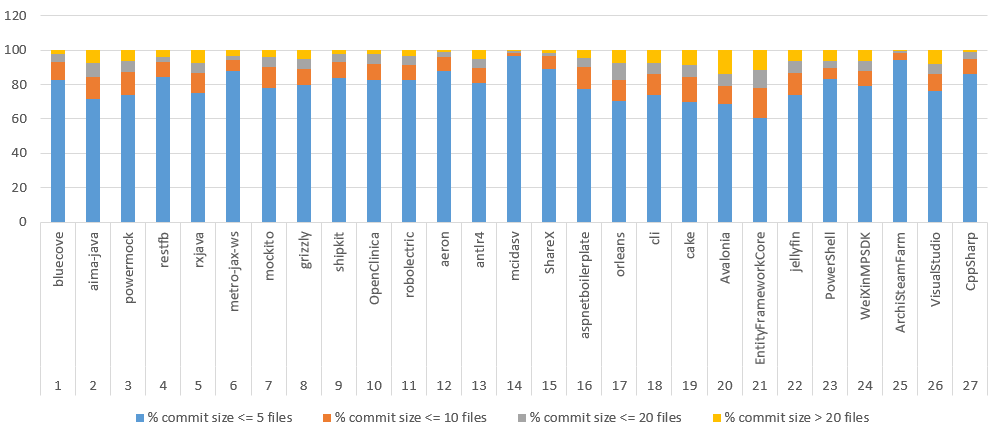
\includegraphics[width=\textwidth]{commit_distribution.png}
	\caption{\label{fig:fig1} Commit transaction size(cs) trend in percentages.}
     \end{figure}
\end{center}
\end{frame}

%%%%%%%%%%%%%%%%%%%%%%%%%%%%%%%%%%%%%%%%%%%
 \begin{frame}
\frametitle{Filtering based on the size of commit transactions (cont.)}

We also analyzed the number of co-changing pairs extracted from each commit transaction size(cs) group

\begin{center}
     \begin{figure}
	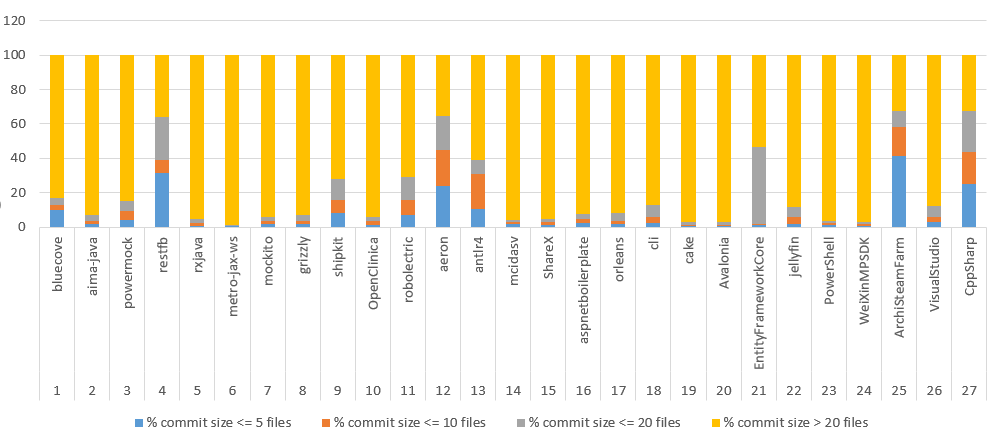
\includegraphics[width=\textwidth]{ld_distribution.png}
	\caption{\label{fig:fig1} Percentages of pairs extracted from each commit transaction size(cs) group}
     \end{figure}
\end{center}
\end{frame}

%%%%%%%%%%%%%%%%%%%%%%%%%%%%%%%%%%%%%%%%%%%
 \begin{frame}
\frametitle{Filtering based on the size of commit transactions (cont.)}

One single commit transaction can lead to a large amount of co-changing pairs. 
 \vskip 0.3cm 
For example in RxJava we have commit transactions with 1030 source code files, this means that those commits can generate 
$\Comb{n}{k}=\frac{n!}{k!(n-k)!} = \frac{1030!}{2!(1028)!} = 529 935$ logical dependencies.
 \vskip 0.3cm 

 By setting a threshold on the commit transaction size we can avoid the introduction of those co-changing pairs into the system.

\end{frame}

%%%%%%%%%%%%%%%%%%%%%%%%%%%%%%%%%%%%%%%%%%%
 \begin{frame}
\frametitle{Filtering based on number of occurrences}
One occurrence of a co-change pair can be a coincidence. To avoid this kind of coincidences, we set a minimum number of
repeated occurrences for a co-change to be counted as logical dependency. The values for this threshold are 1,
2, 3 and 4.

\end{frame}

%%%%%%%%%%%%%%%%%%%%%%%%%%%%%%%%%%%%%%%%%%%
 \begin{frame}
\frametitle{Filtering based on number of occurrences (cont.)}

\begin{center}
     \begin{figure}
	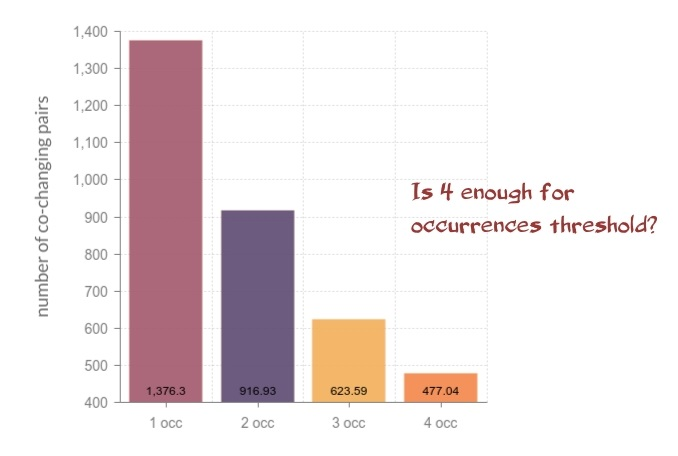
\includegraphics[scale=0.45]{occ2.jpg}
	\caption{\label{fig:fig1}The average number of co-changing pairs after occurrence filtering.}
     \end{figure}
\end{center}
If we try to go higher with the occurrences threshold, we will risk filtering all the existing co-changing pairs for some systems.
\end{frame}

%%%%%%%%%%%%%%%%%%%%%%%%%%%%%%%%%%%%%%%%%%%
 \begin{frame}
\frametitle{Filtering based on connection strength}

This filter focuses on the connection strength of a co-changing pair (how strongly connected are the entities that form a co-changing pair).
Assuming that we have a co-changing pair formed by entities A and B:
\begin{equation}
 connection\ factor\ for\ A = \frac{100 * commits\ involving\ A\ and\ B}{total\ nr\ of\ commits\ involving\ A}
\end{equation}

\begin{equation}
 connection\ factor\ for\ B = \frac{100 * commits\ involving\ A\ and\ B}{total\ nr\ of\ commits\ involving\ B}
\end{equation}
\end{frame}

%%%%%%%%%%%%%%%%%%%%%%%%%%%%%%%%%%%%%%%%%%%
 \begin{frame}
\frametitle{Filtering based on connection strength (cont.)}

The co-changing pairs are filtered out based on two scenarios:
\begin{itemize}
	\item factor A and factor B $\geq threshold \%$ 
	\item factor A or factor B $\geq threshold \%$ 
\end{itemize}
 \vskip 0.3cm 
We begin with a threshold value of 10 and increment it by 10 until we reach 100. 

\end{frame}

%%%%%%%%%%%%%%%%%%%%%%%%%%%%%%%%%%%%%%%%%%%
 \begin{frame}
\frametitle{Filtering based on connection strength (cont.)}

\begin{center}
     \begin{figure}
	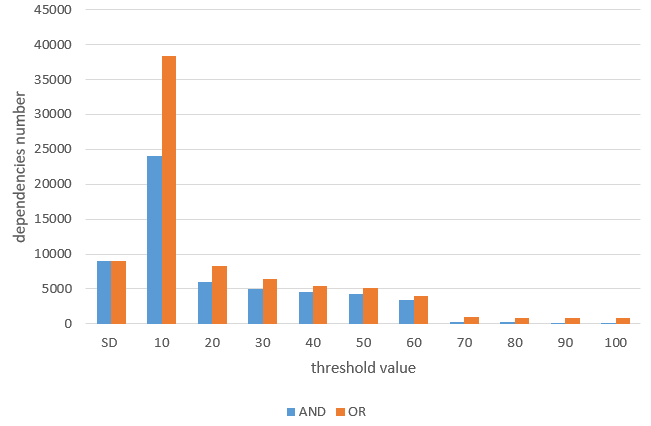
\includegraphics[width=\textwidth]{strength_results.PNG}
	\caption{\label{fig:fig1} The average number of co-changing pairs after connection strength filtering.}
     \end{figure}
\end{center}

If we filter out all the co-changing pairs that do not update at least half of the
time together (factor A and factor B ≥ 50\% ) we remain with a decent quantity of co-changing pairs.

\end{frame}


%%%%%%%%%%%%%%%%%%%%%%%%%%%%%%%%%%%%%%%%%%%
 \begin{frame}
\frametitle{Overlaps between structural and co-changing pairs}

\begin{center}
     \begin{figure}
	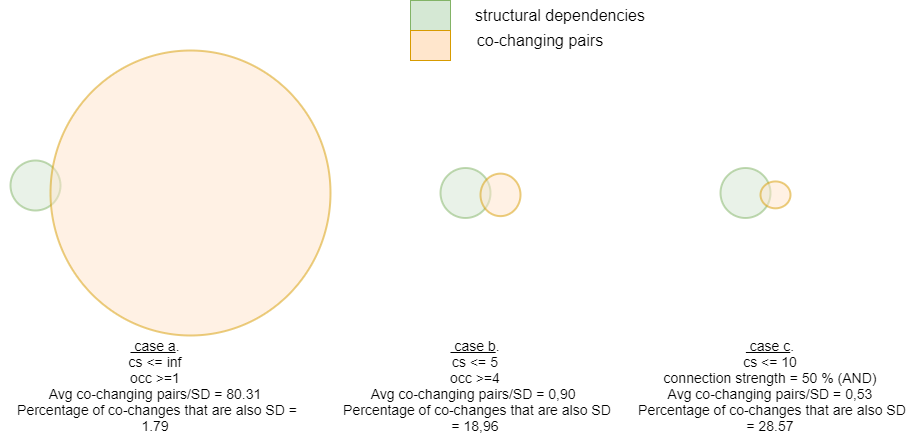
\includegraphics[scale=0.35]{figvenn_OVERLAPP.png}
     \end{figure}
\end{center}

\end{frame}


%%%%%%%%%%%%%%%%%%%%%%%%%%%%%%%%%%%%%%%%%%%

 \begin{frame}
\frametitle{Conclusions}
In order to identify logical dependencies from co-changing pairs we apply 3 sorts of filters: the commit size filter, occurrence filter, and connection strength filter. 
 \begin{itemize}
        \item  the commit size filter is used to reduce the quantity of co-changing pairs extracted
        \item  the occurrence and connection strength filter are used to increase the confidence that the co-changing pairs are logical connected
	\begin{itemize}   
        \item  the occurrence filter is not suited for systems of medium and small size
	\item  the connection strength filter is better suited for all systems sizes and we remain with a decent quantity of co-changing pairs after filtering
    	\end{itemize}
    \end{itemize}
\begin{block}{Future work}
For future investigations regarding the usage of the dependencies extracted we will use the commit size filter with threshold 10 combined with the connection strength filter.
\end{block}
\end{frame}

%%%%%%%%%%%%%%%%%%%%%%%%%%%%%%%%%%%%%%%%%%%
 \begin{frame}
\frametitle{Articles published}
Based on the research presented we published two articles:
\begin{itemize}
\item Adelina Diana Stana. and Ioana Sora.  \textit{Identifying logical dependencies from
co-changing classes.} In Proceedings of the 14th International Conference on
Evaluation of Novel Approaches to Software Engineering - Volume 1: ENASE,,
pages 486–493. INSTICC, SciTePress, 2019.


\item Stana Adelina and Sora Ioana. \textit{Analyzing information from versioning systems
to detect logical dependencies in software systems.} In International Symposium
on Applied Computational Intelligence and Informatics (SACI), May 2019.
\end{itemize}
\end{frame}

%%%%%%%%%%%%%%%%%%%%%%%%%%%%%%%%%%%%%%%%%%%

\end{document}
